\chapter {OSCAD on Aakash}
\label{chap11}

Aakash provides great platform for learning and education. With
GNU/Linux now running on Aakash, most of our student developers will
find it useful. \index{Aakash}The best part is, almost all GNU/Linux applications
runs on Aakash. As tools such as KiCad, Ngspice and Scilab are already
running on Aakash, OSCAD installation procedure is similar to any
other desktop running GNU/Linux. With OSCAD running of Aakash, it
proves Aakash's capability to run Electronic design tools. It also
shows OSCAD's portability from desktops to hand held devices.

%Figure \ref{fig: Oscad Website} is shown below.\\
\begin{figure}[h!]
\centering
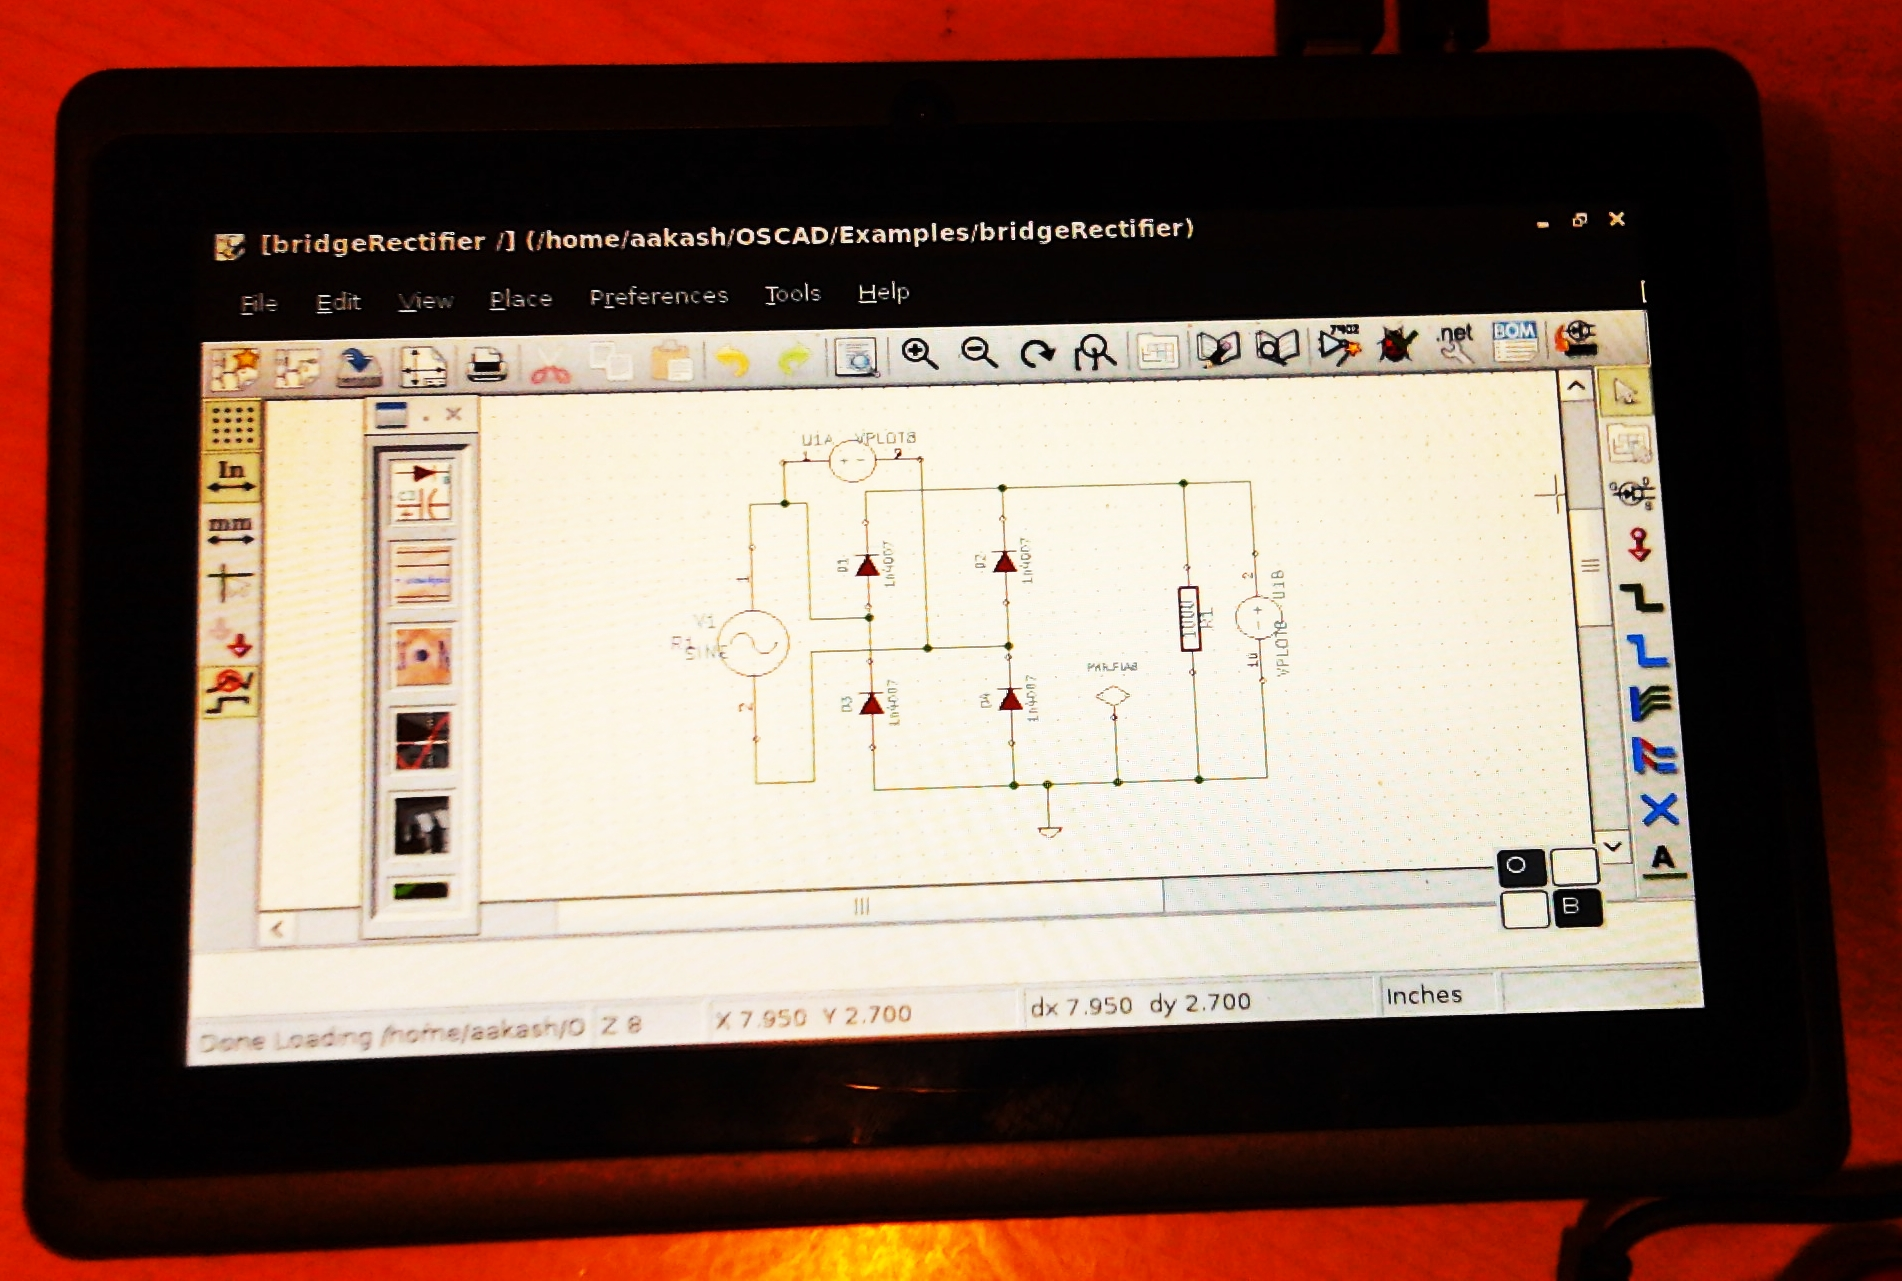
\includegraphics[width=0.9\textwidth]{figures/aakash_br.png}
\caption{Bridge rectifier schematic on Aakash}
\label{fig: Bridge rectifier schematic on Aakash}
\end{figure}


\section{Installation}

Installation of OSCAD is similar to its GNU/Linux desktop, please
follow the same instructions mentioned in Chapter 2. OSCAD installer
runs {\tt Synaptic package manager} underneath. This package manager
is smart enough to detect your CPU architecture. It downloads and
install specific packages to your machine architecture. We are
further enhancing the installer so that it could download required
version of Scilab for specific machine architecture from the internet
with minimum user intervention.

One has to ensure that his/her Aakash tablet is connected to the
internet through \emph{WiFi} before starting the installation
procedure. OSCAD is currently in development stage on Aakash, but it
is completely usable. Once it is ready for Aakash, it will come
preinstalled on Aakash.

\begin{figure}[h!]
\centering
\includegraphics[width=0.9\textwidth]{figures/aakash_ngspice.png}
\caption{Ngspice running on Aakash}
\label{fig: NgSpice running on Aakash}
\end{figure}

\section{Porting on Aakash}

The design framework of OSCAD made it extremely simple to run it on
Aakash with minimum modification. As OSCAD was initially developed on
an Ubuntu distribution which has GNOME-terminal primarily. This
GNOME-terminal was called whenever there was a need for user input
using terminal.

On the other hand, GNU/Linux side of Aakash also uses same Ubuntu
desktop version but not GNOME as it Desktop Environment. To be ease on
memory and CPU it uses LXDE desktop environment. LXDE is intended for
systems with low memory and CPU. LXDE on the other side has
LX-terminal which made it difficult for OSCAD process to invoke
terminal on demand. Keeping in mind the portability issue, we have
dropped both GNOME and LX terminal. Instead we have now opted for {\tt
  xterm} which is the standard \emph{terminal emulator} for X-Window
System. 

\begin{figure}[h!]
\centering
\includegraphics[width=0.9\textwidth]{figures/aakash_setup.png}
\caption{OSCAD running with external keyboard and mouse attached}
\label{fig: OSCAD running with external keyboard and mouse attached}
\end{figure}

\section{Usage}

Advantage of using OSCAD on Aakash is its portability and
performance. Beside having touch on Aakash, one may attach external
keyboard and mouse. One should find the similar interface of OSCAD on
Aakash as its Desktop version. Sometimes keyboard shortcuts are more
handy than using touch controls when running designing and simulation
tool.


